\chapter{ValleyHall}
\section{Berry curvature in Gapped graphene}

The Hamiltonian for the gapped graphene near the point $K_1$ and $K_2$ can be written as 
\begin{equation}
    H_{K_1}=H_{K_2}^\dagger=
    \begin{bmatrix}
        \Delta & \hbar v_F(k_x+ik_y)\\
        \hbar v_f(k_x-ik_y)& \Delta
    \end{bmatrix}
\end{equation}
Where $\Delta$ is the energy gap and $v_F$ is the Fermi velocity. For ease of notation we are going to work with just $H_{K_1}$ and drop the $K_1$,\footnote{Don't worry, I'll bring it back if when we'll need it} and for ease of computation we define $\vect q=\hbar v_F\vect k$
\begin{equation}
    H=
    \begin{bmatrix}
        \Delta & q_x+iq_y\\
        q_x-iq_y& \Delta
    \end{bmatrix}=
    \sigma_x q_x + \sigma_y q_y + \sigma_z \Delta \equiv  \boldsymbol \sigma \cdot \vect E
\end{equation}

Here the enegry vector $\vect E$ is defined as $\vect E =( q_x,q_y,\Delta)$. The nice things about it is that $E=|\vect E|=\sqrt{q_x^2+q_y^2+\Delta^2}$ is the positive eigenvalue of the hamiltonian (the negative eigenvalue is just $-E$).\newline
To calculate the Berry curvature we are first going to calculate the Berry connection \ref{eq:connection}, and to calultate the Berry connection we need the eigenvectors which are well known for the Hamiltonian of the form $\boldsymbol \sigma \cdot \vect{E}$.

\begin{equation}
    \ket{+;\theta,\phi}=
    \begin{bmatrix}
        \cos{\frac \theta 2}\\
        e^{i\phi}\sin{\frac \theta 2}
    \end{bmatrix}
    \quad
    \ket{-;\theta,\phi}=
    \begin{bmatrix}
        -e^{-i\phi}\sin{\frac \theta 2}\\
        \cos{\frac \theta 2}
    \end{bmatrix}
\end{equation}
Where $\theta$ and $\phi$ are the coordinates of $\vect E$ in the polar representation

Now we can calculate the Berry connection

\begin{equation}
    A_\theta^+=-A_\theta^-=0 \quad A_\phi^+=-A_\phi^-=\sin^2\frac \theta 2
\end{equation}

This means that the Berry curvature is
\begin{equation}
    \Omega^+_{\theta\phi}=-\Omega^-_{\theta\phi}=\partial_\theta A^+_\phi=\frac{\sin \theta}2
\end{equation}

From now on we are going to work with $\Omega^+$ and we are going to drop the $+$ sign to make the notation lighter.

We want to express $\Omega$ in terms of $\vect q$, however it's more convenient to write it in terms fo  $\cos \theta$ and $\phi$, so we do a small coordinate transformation


\begin{equation}
    \Omega_{\theta\phi}=\frac{\partial\cos\theta}{\partial \theta}\Omega_{\cos(\theta)\phi} \rightarrow \Omega_{\cos(\theta)\phi}=\frac 12
\end{equation}



Now we can easily make the transformation to express $\Omega$ in terms of $\vect q$. The Berry curvature transforms like any other tensor under coordinate transformation, so

\begin{equation}
    \Omega_{q_xq_y}=\frac{\partial\cos \theta}{\partial q_x}\frac{\partial \phi}{\partial q_y}\Omega_{\cos(\theta)\phi}+\frac{\partial \phi}{\partial q_x}\frac{\partial\cos \theta}{\partial q_y}\Omega_{\phi\cos(\theta)} 
\end{equation}

That can be rewritten as

\begin{equation}
    \Omega_{q_xq_y}=\frac 12 \det\bigg[\frac{\partial (cos\theta,\phi)}{\partial (q_x,q_y)}\bigg]=\frac 12 \frac{\Delta^2}{q^2E^3}(q_x+q_y-2q)
\end{equation}


And finally we can express it in terms of $\vect k$
\begin{equation}
    \Omega_{k_xk_y}=(\hbar v_F)^2\Omega_{q_xq_y}=\frac {\hbar v_F}2 \frac{\Delta^2}{k^2E^3}(k_x+k_y-2k)
\end{equation}
Up until now we have worked with the Hamiltonian $H_{K_1}$, but with the $K_1$ hidden. The Berry curvature around $K_2$ is equal, but with opposite sign (figure \ref{fig:cones})
\footnote{
    A short proof for it can be the following: If we send $k_y\to -k_y$ we effectively send $H_{K_1}\to H_{K_2}$.\\
    The berry curvature can be written as $\Omega_{k_xk_y}=i\bra{\partial _{k_x}n}\wedge\ket{\partial_{k_y}n}$. By sending  $k_y\to -k_y$ we have that $\Omega\to-\Omega$.}

\begin{figure}
    \centering
    \includegraphics[width=0.7\linewidth]{Immagini/ValleyHall/band_graphene.pdf}
    \includegraphics[width=0.7\linewidth]{Immagini/ValleyHall/curvature_graphene.pdf}
    \caption{In the top panel are displayed the Energy bands in 2D. In the bottom panel with the dotted line are displayed a section of the energy bands, and with the continuous red line the Berry curvature.}
    \label{fig:cones}
\end{figure}









 

\section{Valley-Hall effect}
The Hall conductivity $\sigma_{xy}$ is 
\begin{equation}
    \sigma_{xy}=\frac{e^2}\hbar \int_{\mathbb R^2} f[E^+(k)]\Omega^+_{k_xk_y}+f[E^-(k)]\Omega^-_{k_xk_y}\frac{d^2\vect k}{2\pi}
    \label{eq:valley-conductivity-1}
\end{equation}
Where $f(E)=\big[e^{\beta (E-\mu)}+1\big]^{-1}$ is the Fermi-Dirac distribution, it is applied once for the states with positive energy and once for the states with negative energy.

We are going to analyze the system at low temperatures ($k_\beta T\ll 1$), so our Fermi-Dirac distribution can be considered like a step-function.

First let's integrate the conductivity for the positive energies and drop the $+$ sign to make the notation lighter.

\[
    \int_{\mathbb R^2} f[E(k)]\Omega_{k_xk_y}dk_xdk_y=\int_{\mathbb R^2} f[E(q)]\Omega_{q_xq_y}dq_xdq_y\approx
\]

\[
    \approx\int_{0}^{2\pi}\int_{0}^{q_F}\frac12 \frac{\Delta^2}{q^2E^3}(q_x+q_y-2q)qdqd\theta=
\]

\[
    =-2\pi\Delta^2\int_0^{q_f}\frac{dq}{E^2} =-2\pi\Delta^2\int_0^{q_f}\frac{dq}{(\Delta^2+q^2)^{3/2}}= 
    -\frac{2\pi q_F}{\sqrt{\Delta^2+q_F^2}}
\]

And now we express it in terms of the chemical potential $\mu$ \footnote{Here we can use interchangeably $\mu$ and $E_F$}


\begin{equation}
    \int_{\mathbb R^2} f[E(k)]\Omega_{k_xk_y}dk_xdk_y\approx-2\pi \frac{\sqrt{\mu^2-\Delta^2}}\mu\theta(\mu-\Delta)
\end{equation}
The $\theta(\mu-\Delta)$ is there to make sure that if no states are inside the Fermi-Dirac the integral is zero. One thing to notice is that if you have $\mu \gg \Delta$ (aka. all states in the band are occupied) then the integral is equal to $-2\pi$. The integral of the lower band is very similar. By the end equation of the conductivity \ref{eq:valley-conductivity-1} becomes
\begin{equation}
    \sigma_{xy}(\mu)=-\frac {e^2}{2\pi \hbar}\Bigg[\frac{\sqrt{\mu^2-\Delta^2}}{\mu} \theta(\mu^2-\Delta^2) - \theta(\mu-\Delta)\Bigg]
    \label{eq:valley-conductivity-2}
\end{equation}
\begin{figure}
    \centering
    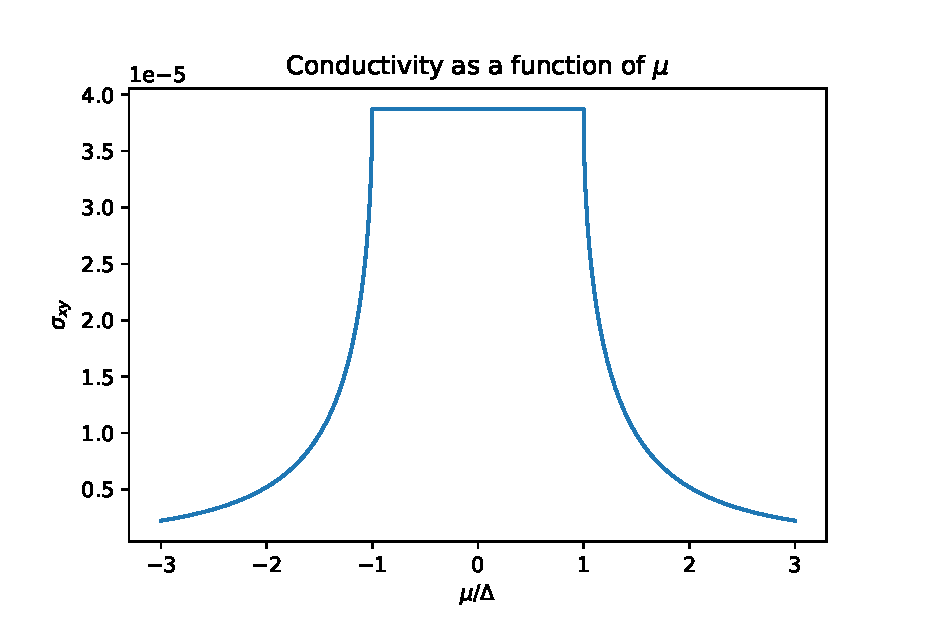
\includegraphics[width=\linewidth]{Immagini/ValleyHall/sigma_xy.eps}
    \caption{Here is shown $\sigma_{xy}(\mu)$ (eq. \ref{eq:valley-conductivity-2}). Notice how, when $\mu \in [-\Delta,\Delta]$ then $\sigma_{xy}=\frac {e^2}{2\pi \hbar}$}
    \label{fig:sigma_xy}
\end{figure}
To be fear we only calculated $\sigma_{xy}$ for the electrons in the valley $K_1$, the conductivity for the other valley is just $-\sigma_{xy}$. So, putting it all together, we have

\begin{equation}
    \sigma_{K_i,xy}(\mu)=(-1)^i\frac {e^2}{2\pi \hbar}\Bigg[\frac{\sqrt{\mu^2-\Delta^2}}{\mu} \theta(\mu^2-\Delta^2) - \theta(\mu-\Delta)\Bigg]
    \label{eq:valley-conductivity-complete}
\end{equation}
However in most cases it's safe to assume that the chemical potential is inside the energy gap, so equation \ref{eq:valley-conductivity-complete} becomes
\begin{equation}
    \sigma_{K_i,xy}=(-1)^{i+1}\frac {e^2}{2\pi \hbar}
\end{equation}



\section{Non-local Charge transport}
If we apply a voltage $V$ in two opposite points of a strip of a ohmic material of width $W$ and infinite lenght, and  we see a current that flows from one point to another figure \ref{fig:beconcini_strip}.\newline
\begin{figure}
    \centering
    \includegraphics[width=0.7\linewidth]{Immagini/ValleyHall/beconcini_strip.pdf}
    \caption{Representation of the strip}
    \label{fig:beconcini_strip}
\end{figure}
Clearly the current isn't completely localized along the axis that unites the two injection points, and so does the voltage difference.\newline
If we probe the voltage from two different points with an offset of $x$ from the injection points and we divide it by the total current between the contacts we see that  

\begin{equation}
    \frac{V(x)}I=\frac{2\rho}\pi\ln\bigg |\coth \Big(\frac{\pi x}{2W}\Big)\bigg |
\end{equation}
Where $\rho$ is the resistivity. Don't worry later on there is the proof of this equation.\newline

However, two-dimentional material like gapped graphene \cite{gorbachev2014detecting,sui2015gate,shimazaki2015generation} and transition metal dichalcogenides \cite{xiao2012coupled,mak2014valley,lee2017valley}, don't obey this equation. This is because theese materials display the Valley Hall effect we talked about previously (inserire reference a sezione).

Non-local transport can be a useful tool to probe the existance of anomalous Hall effect \cite{valenzuela2006direct,abanin2009nonlocal,brune2010evidence,abanin2011giant,balakrishnan2013g,wang2015proximity}


\section{Theory of non local charge transport}

The charges inside the material get pushed around from the electrochemical potential $\psi_K$


\begin{equation}
    \psi_{K}(\vect r)= V(\vect r)-\frac 1e \mu_K[n_{K_1}(\vect r),n_{K_2}(\vect r),T]
\end{equation}

Where $\phi$ is the electrical potential, and $\mu_K=\frac {\partial}{\partial n_{K}}F[n_{K_1}(\vect r),n_{K_2}(\vect r),T]$ is the chemical potential of the material and $F$ is the free energy.

The current generated from this potential in the valley $K_\alpha$ in the $i-$th direction is

\begin{equation}
    -eJ_{K_\alpha,i}(\vect r)= \sum_{j,b} \underbrace{-\sigma_{K_\alpha K_\beta ,ij}}_{\textrm{conductivity}}\partial_j\psi_{K_\beta }(\vect r)
\end{equation}
From now we are going to set $T\approx 0$\footnote{A more precise statement is that the thermal De Broglie wavelenght $\lambda_T$ must be much larger than the average distance between the electrons. We are not going into the math here, but if you want to calculate it, keep in mind that the dispersion relation is relativistic, so the formula of $\lambda_T$ is going to be a bit different}
and ignore intervalley scattering, so if $K_\alpha \neq K_\beta $ $\sigma_{K_\alpha K_\beta ,ij}=0$, also because of this the free energy can be written as the sum of the two Free energies
\begin{equation}
    F(n_{K_1},n_{K_2})=F_1(n_{K_1}(\mathbf r))+F_2(n_{K_2}(\mathbf r))
\end{equation}
And so the chemical potential of a given valley depend only on the number of electron in the same valley
\begin{equation}
    \mu_\alpha(n_{K_\alpha}(\mathbf r))=\frac{\partial}{\partial n_{K_\alpha}}F(n_{K_0},n_{K_1})=\frac{\partial}{\partial n_{K_\alpha}}F_\alpha(n_{K_\alpha}(\mathbf r))
\end{equation}
This simplifies the trasport equation in 

\begin{equation}
    -e\mathbf J_{K_{\alpha}}(\mathbf r)= \sigma_{K_\alpha}(\mathbf r)\nabla \psi_{K_\alpha}(\mathbf r)
    \label{eq:current-1}
\end{equation}
Where $\sigma_{K_\alpha}$ is the following matrix
\[
    \sigma_{K_\alpha}=
    \begin{bmatrix}
        \sigma_{K_\alpha K_\alpha,xx} & \sigma_{K_\alpha K_\alpha,xy}\\
        -\sigma_{K_\alpha K_\alpha,xy}^* & \sigma_{K_\alpha K_\alpha,xx}
    \end{bmatrix}
\]
Now we need to write the gradient electrochemical potential $\nabla \psi(\vect r)$
\begin{equation}
    \nabla \psi_{K_\alpha}(\mathbf r)=\nabla V(\mathbf r) -\frac 1e \frac{\partial}{\partial n_{K_\alpha}}\mu_\alpha(n_{K_\alpha}(\mathbf r))\nabla n_{K_\alpha}
    \label{eq:echemical1}
\end{equation}
From equation INSERIRE REFERENCE A EQUAZIONE we can write for gapped Dirac hamiltonians that VERIFICARE SE VALE ANCHE PER BILAYER GRAPHENE  \[\frac{\partial \mu_{K_\alpha}}{\partial n_{K_\alpha}}=\frac{\pi}{\sqrt{2\pi |n|+\Delta^2}}+\Delta\delta(n)\approx \frac \pi\Delta +\Delta\delta(n) \quad \forall \alpha\]
In this equation we assumed that there are very few charge carries, so $\frac n{\Delta^2}\approx 0$. We can shorten the equation \ref{eq:echemical1} by defining
\begin{equation}
    e^2D_{K_\alpha,ij}=\sigma_{K_\alpha, ij}\frac{\partial \mu_\alpha}{\partial n_{K_\alpha}}[n_{K_\alpha}(\mathbf r)]
\end{equation}
So equation \ref{eq:current-1} becomes

\begin{equation}
    -eJ_{K_\alpha,i}(\mathbf r)=\sigma_{K_\alpha, ij}E_j(\mathbf r) -eD_{K_\alpha,ij}\partial _jn_{K_\alpha}(\mathbf r)
\end{equation}
or, written in matrix form
\begin{equation}
    -e\mathbf J_{K_\alpha}(\mathbf r)=\sigma_{K_\alpha}\mathbf E(\mathbf r) -eD_{K_\alpha}\nabla n_{K_\alpha}(\mathbf r)
\end{equation}
Where $\sigma_{K_\alpha}$ and  $-eD_{K_\alpha}$ are matrices.

\subsection{Re-writing the equations in terms of charge current and valley current}
Measuring the currents in different valley can be cumbersome, however measuring the charge current $\mathbf J_{c}=\mathbf J_{K_1}+\mathbf J_{K_2}$ is straightforward, and for mathematical convenience we also define the valley current $\mathbf J_{v}=\mathbf J_{K_1}-\mathbf J_{K_2}$.

Since we no longer describe the currents in terms of their valley index, but on the sum and the difference of what happens at the different valleys, we are going to reparametrize also the other quantities in the same fashion.


\begin{equation}
    \begin{cases}
        \sigma_c=\sigma_{K_1}+\sigma_{K_2}=2\sigma_{xx}\delta_{ij}\\
        \sigma_v=\sigma_{K_1}-\sigma_{K_2}=\sigma_v=2\sigma_{xy}\epsilon_{ij}
    \end{cases}
\end{equation}
The term $-eD_{K_\alpha}\nabla n_{K_\alpha}(\mathbf r)$ is a little harder to traslate. First off we are going to impose the local charge conservation

\[
    n(\mathbf r)=n_{K_0}+n_{K_1}\approx 0
\]
and so 

\begin{equation}
    n_v(\mathbf r)=n_{K_1}-n_{K_2}=2n_{K_1}=-2n_{K_2}
\end{equation}
Now let's do the sum of the $D_{K_\alpha}\nabla n_{K_\alpha}(\mathbf r)$ terms to write them in terms of charge and valleys degrees of freedom

\[D_{K_1}\nabla n_{K_1}+D_{K_2}\nabla n_{K_2}=(D_{K_1}-D_{K_2})\nabla n_v(\mathbf r)/2\]

\[D_{K_1}-D_{K_2}=\sigma \frac{\partial \mu_1}{\partial n_{K_1}}- \sigma^T \frac{\partial \mu_2}{\partial n_{K_2}}\]
since $\mu_v=2\mu_1=-2\mu_2$ and $n_v=2n_{K_1}=-2n_{K_2}$

\[D_{K_1}-D_{K_2}=\frac 1{e^2}(\sigma-\sigma^T)\frac{\partial \mu_v}{\partial n_v}=\frac 2{e^2}\sigma_v\frac{\partial \mu_v}{\partial n_v}\]
so I define 

\[D_{cv}=\frac 2{e^2}\sigma_v\frac{\partial \mu_v}{\partial n_v}\approx\frac 2{e^2} \frac \pi\Delta\sigma_v\]
so we get that

\[D_{K_1}\nabla n_{K_1}+D_{K_2}\nabla n_{K_2}=D_{cv}n_v\]
Putting it all together we have that

\[\mathbf J_c(\mathbf r)=\sigma_c \mathbf E(\mathbf r)+eD_{cv}\nabla n_v(\mathbf r)\]
Writing all the indices

\[J_{c,i}=\sum_j \sigma_{c,xx}\delta_{ij}E_i+D_{cv,xy}\epsilon_{ij}\partial_j n_v\]
so we can rewrite them as

\[\mathbf J_{c}= \sigma_{c,xx}\mathbf E_i + D_{cv,xy} \nabla \times n_v\]
where $\sigma_{c,xx}$ and $D_{cv,xy}$ are scalars

